\documentclass{article}[12pt]
\renewcommand{\baselinestretch}{1.5}
\setlength{\parskip}{1em}

\usepackage[parfill]{parskip}
\usepackage[affil-it]{authblk}
\usepackage[space]{grffile}

\usepackage[a4paper]{geometry}
\geometry{verbose}
\usepackage{float}
\usepackage{graphicx}
\graphicspath{{figures/}}
\usepackage{setspace}
\usepackage{caption}

\usepackage[utf8]{inputenc}
\usepackage[english]{babel}

\usepackage{latexsym,textcomp,longtable,tabulary}
\usepackage{booktabs,array,multirow,braket}
\usepackage{amsfonts,amsmath,amssymb,mathbbol,calc}
\usepackage{subfigure,color,blindtext,enumitem,siunitx}
\usepackage[dvipsnames]{xcolor}

\usepackage[colorinlistoftodos]{todonotes}

\usepackage{mathtools}
\usepackage{url,hyperref,etoolbox}
\numberwithin{equation}{section}
\hypersetup{colorlinks=false,pdfborder={0 0 0}}

%+figure layout options
\restylefloat{figure}
\setlist{leftmargin=*,before=\setlength{\rightmargin}{\leftmargin}}
%-figure layout options

\providecommand\citet{\cite}
\providecommand\citep{\cite}
\providecommand\citealt{\cite}

\makeatletter
\makeatother

\def\code#1{\texttt{#1}}
\begin{document}

\title{
Nonequilibrium Molecular Dynamics
}

\author{Gregory Szep}
\affil{King's College London}
\date{\today}
\maketitle

\section{scientific publication}
Select a scientific publication about non-equilibrium molecular dynamics of
biomolecules and discuss its relevance respect to the course you attended and
this research assignment.
\pagebreak
\section{Unfolding proteins with umbrella sampling}

\subsection{Structure and unfolding of $\alpha$-helix and $\beta$-hairpin}
Umbrella sampling is a technique in molecular dynamics with which one can
efficiently estimate the free energy surface $E(r)$ of a molecule --- referred to as the
\textit{potential of mean force} along a chosen reaction coordinate $r$. The
reaction coordinate $r$ is typically a nonlinear function of a large configuration
space $x\in\mathbb{R}^M$.
\\\\
To enhance sampling in the reaction coordinate $r$, an artifical \textit{umbrella
potential} $V(r)$ is added to the native classical force fields $U(x)$ to bias the molecule
configuration $x$ towards a fixed value of the reaction coordinate $r=f(x)$.
The molecule is allowed to explore the configuration space $x$ in the vicinity of
this value and the \textit{potential of mean force} is estimated from the resulting
trajectory, which is treated as an ergodic ensemble. For finite temperature $\beta$
\begin{align}
	E(r)= -\frac{1}{\beta}\ln\big\langle
	\delta\left(r-f(x)\right)
	\big\rangle_{U(x)+V\circ f(x)}
		-V(r)
		+\mathrm{const}
\end{align}
Empirically the expectation $\langle\delta\left(r-f(x)\right)\rangle_{U(x)+V\circ f(x)}$
is nothing but the histogram of $r$ over a trajectoy biased by a fixed $V(r)$. This
locally estimates $E(r)$. For a sufficiently highly resolved grid in $r$ these
local estimates can be vertically aligned to form a global estimate of $E(r)$.
Highly resolved $r$-grids require more molecular dynamics runs and thus
are computationally expensive. The weighted histogram analysis method (WHAM)
is used to estimate intermediate values of $E(r)$ given a lower resolution grid,
whos $r$ histograms still sufficiently overlap.
\\\\
In the case of unfolding of the $\alpha$-helix and $\beta$-hairpin
the reaction coordinate is the end-to-end distance of the protein. A harmonic
potential is used to keep the ends of the protein a fixed distance apart for
each ensemble. We expect the breaking of bonds and deformation of structure
as $r$ increases.
Figure \ref{fig:unfold} reveals the structure of typical conformations of both
proteins for ensembles along the reaction coordinate and Figure \ref{fig:hydrogen}
quantifies unfolding in terms of the histograms of intra-protein hydrogen bonds
$n(r)$ with respect to local histograms of $r$.

\begin{figure}[H]
	\centering{}
	\captionsetup{justification=centering}
	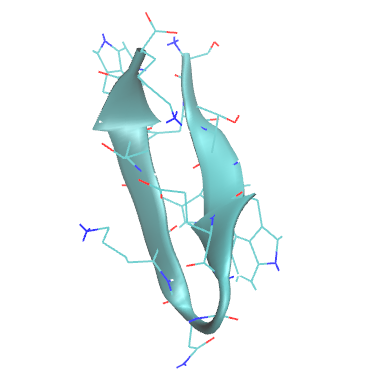
\includegraphics[scale=0.21]{hairpin-1}
	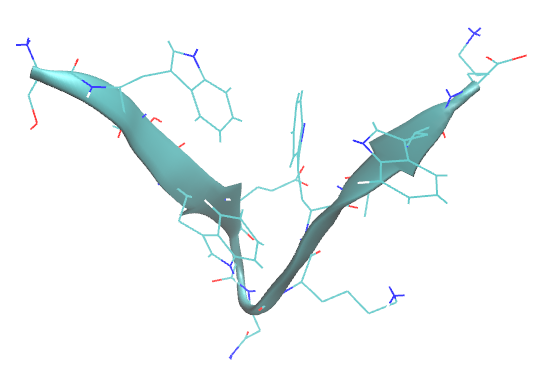
\includegraphics[scale=0.21]{hairpin-2}
	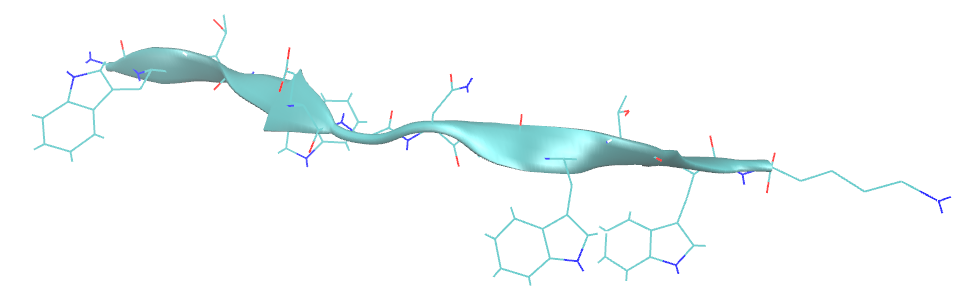
\includegraphics[scale=0.21]{hairpin-3}
	\includegraphics[scale=0.35]{helix-1}
	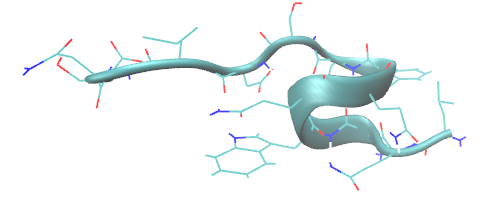
\includegraphics[scale=0.35]{helix-2}
	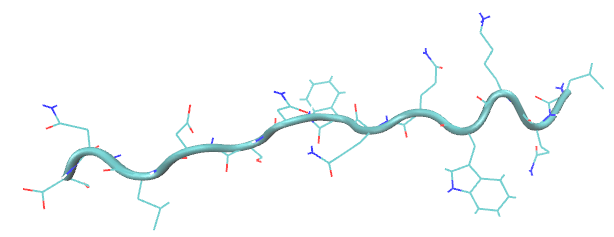
\includegraphics[scale=0.35]{helix-3}
\caption{Structures of $\beta$-hairpin (top) and $\alpha$-helix (bottom)
from\\ ensembles of increasing reaction coordinate from left to right}
\label{fig:unfold}
\end{figure}
\begin{figure}[H]
	\centering{}
	\captionsetup{justification=centering}
	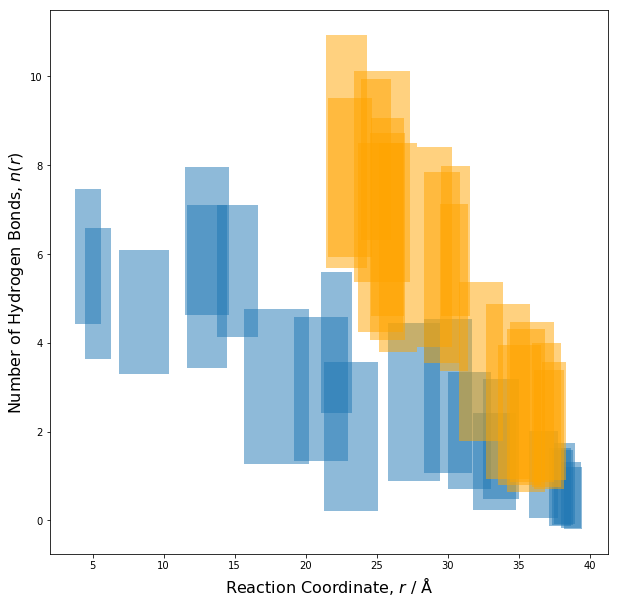
\includegraphics[scale=0.5]{hydrogen}
\caption{Boxes represent biased ensembles of $\color{NavyBlue}{\beta\mathrm{-hairpin}}$ and
$\color{orange}{\alpha\mathrm{-helix}}$\\centered at the means and bounded by standard
deviations of $n(r)$ and $r$}
\label{fig:hydrogen}
\end{figure}
\pagebreak
Figure \ref{fig:hydrogen} reveals the patchy overlap between adjacent ensembles
the reaction coordinate $r$ and its negative correlation with number of hydrogen
bonds $n(r)$. The transient increase in hydrogen bonds in the $\beta$-hairpin at
around $12\mathrm{\AA}$ may indicate a metastable fold state. While the breaking
of a hydrogen bond does contribute to the increase $E(r)$ by
$1-3\mathrm{kcal\,mol^{-1}}$ and may account for an increase of up to
$\sim21\mathrm{kcal\,mol^{-1}}$ as seen in Figure \ref{fig:pmf}, the large
uncertainties do not allow us to confidently say those are the only energetic
contributions. Perhaps contributions may come from the deformation of non-bonded
interactions between residues; this can be confirmed with a Ramachandran plot.

\subsection{Potential mean force and bootstraping}
Bootstrapping is a resampling method that quantifies statistical uncertainty by
dividing the data into $N$ subsets, hence without additional measruements
uncertainty is obtained by \textit{pulling the data up by its own bootstraps}.
By default the \code{g\_wham} code forms subsets with replacement over the
complete histograms along the reaction coordinate \cite{gwham2010}, leaving us
with $N$ as a hyperparameter.
\\\\
This hyperparameter is subject to the bias-variance trade-off. Chooseing a large
$N$ results in relatively unbiased and uncertain estimates, while a small number
of subsets give rise to more certain yet biased estimates. The former is
preferred but comes with a computational cost. According to Figure
\ref{fig:bootstrap} it appears that the uncertainty bounds converge to a fixed
value after around $N\geq20$ so there is little sense in setting $N$ at any
other value than $N=20$.
\\\\
Figure \ref{fig:pmf} shows the increasing potential of mean force $E(r)$ with
platauing regions that coincide with the transient increases in hydrogen bonds
in Figure \ref{fig:hydrogen}. This confirms the existence of metastable states.
The sharp increase in $E(r)$ for the $\beta$-hairpin at $\sim7\mathrm{\AA}$
corresponds to the unpinning of the hairpin, followed by steady deformations
leading to a metastable state, which is followed by further deformations. Finally at
$\sim35\mathrm{\AA}$ the potential becomes harmonic which corresponding to the
stretching of covalent bonds. An artifact at $\sim38\mathrm{\AA}$ for the
$\alpha$-helix can be seen, possibly due to a jump across the periodic boundary
conditions.
\begin{figure}[H]
	\centering{}
	\captionsetup{justification=centering}
	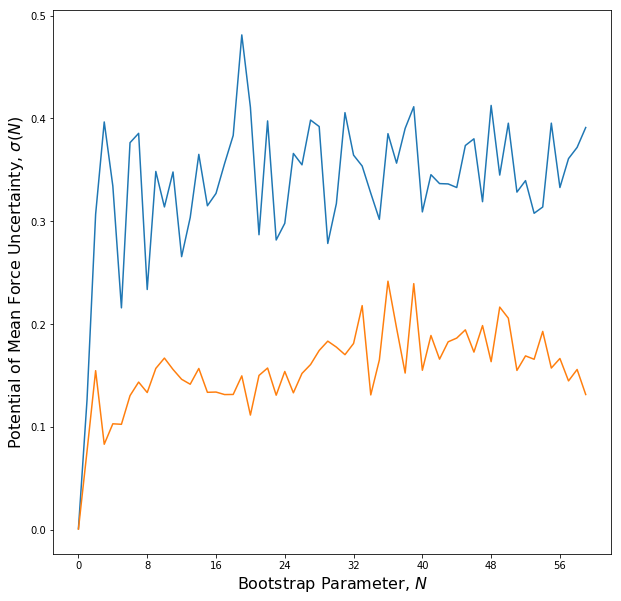
\includegraphics[scale=0.41]{bootstrap}
\caption{Standard deviation of potential of mean force $\sigma(N)$ as a \\function of bootstrap parameter $N$
for the $\color{NavyBlue}{\beta\mathrm{-hairpin}}$ and $\color{orange}{\alpha\mathrm{-helix}}$}
\label{fig:bootstrap}
\end{figure}
\begin{figure}[H]
	\centering{}
	\captionsetup{justification=centering}
	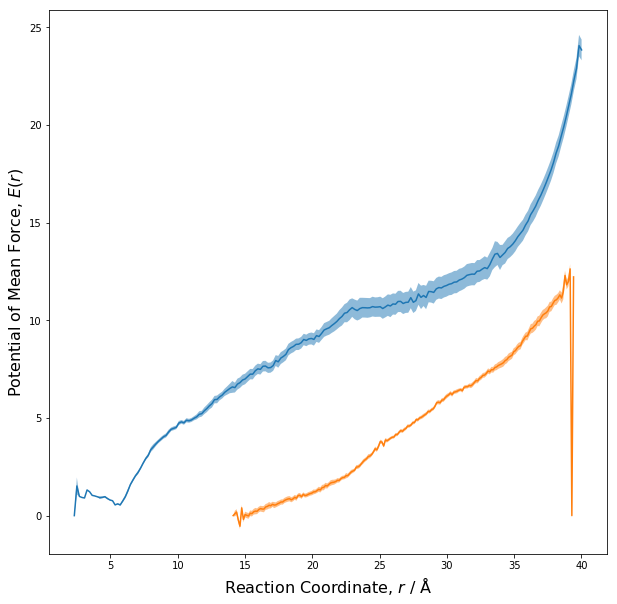
\includegraphics[scale=0.41]{pmf}
\caption{Potential mean force $E(r)$ estimated by WHAM with bootstrap parameter\\$N=20$
as a function of reaction coordinate $r$
for the $\color{NavyBlue}{\beta\mathrm{-hairpin}}$ and $\color{orange}{\alpha\mathrm{-helix}}$}
\label{fig:pmf}
\end{figure}
\section{Conductance of a porin}
\vspace{-5pt}
\subsection{Structure and function}
Porins are $\beta$-barrel transmembrane proteins that act as a pore through
which molecules can diffuse. Outer membrane protein F (ompF) is a nonspecific
weakly cationic selective porin found in \textit{E. Coli} \cite{Novikova2009}.
It is nonspecific in the sense that there is no preference for a particular
chemical species, however it does exhibit weak selective permeability for
cations.
\begin{figure}[H]
	\centering{}
	\captionsetup{justification=centering}
	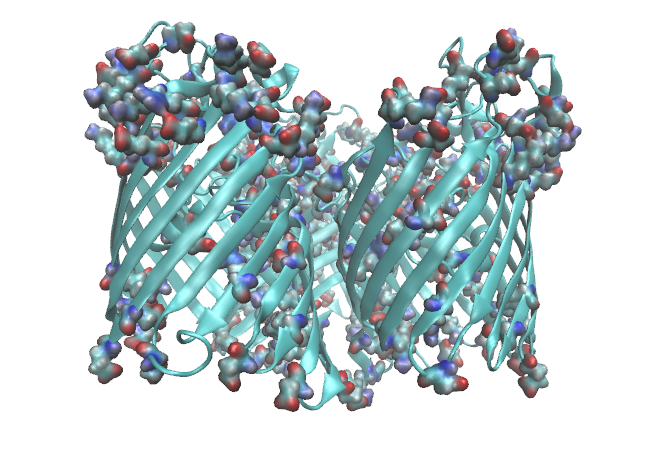
\includegraphics[scale=0.4]{ompf}
\caption{Side-view of ompF: $\beta$-barrel homotrimer forms transmembrane channel.\\
Highlighted are polar residues, which dominanate the outer membrane side.}
\label{fig:ompF}
\end{figure}\noindent
Figure \ref{fig:ompF} shows the structure of ompF: antiparallel $\beta$-strands
forming three barrels that interact locally with neighboring $\beta$-strands, a
long loop inserts into each barrel resulting in channel narrowing, charged
residues form clusters at the entrance to a pore on the outer membrane side as
well as within the narrow channel zone.
\\\\
The narrowing geometry prevents larger potentially harmful molecules such as
detergents from diffusing across the membrane, while allowing small hydrophilic
molecules involved in bacterial metabolism to pass. Charged residues in the
narrowing region of each barrel influence the ion selectivity and permeability
of the channel. Two clusters of oppositely charged residues as shown in Figure
\ref{fig:ompF-charges} generate a screw-like electric field twisted along the
channel axis with a strong transverse component in the pore narrowing region
\cite{Novikova2009}. This field favors cations to pass through the channel.
\begin{figure}[H]
	\centering{}
	\captionsetup{justification=centering}
	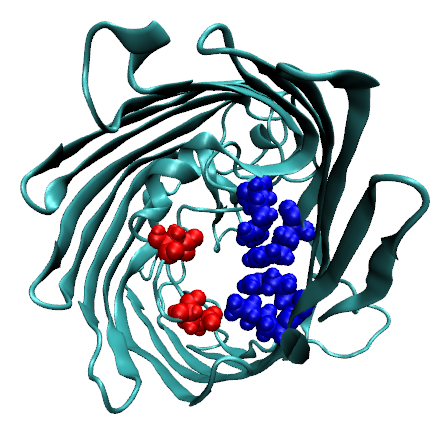
\includegraphics[scale=0.5]{ompf-charges}
\caption{ompF $\beta$-barrel from inner membrane side having residues with
positive \\ $\color{red}{\mathrm{COOH}}$ and negative $\color{blue}{\mathrm{NH_2}}$ partial
charged groups that facilitate cationic selectivity}
\label{fig:ompF-charges}
\end{figure}
\begin{figure}[H]
	\centering{}
	\captionsetup{justification=centering}
	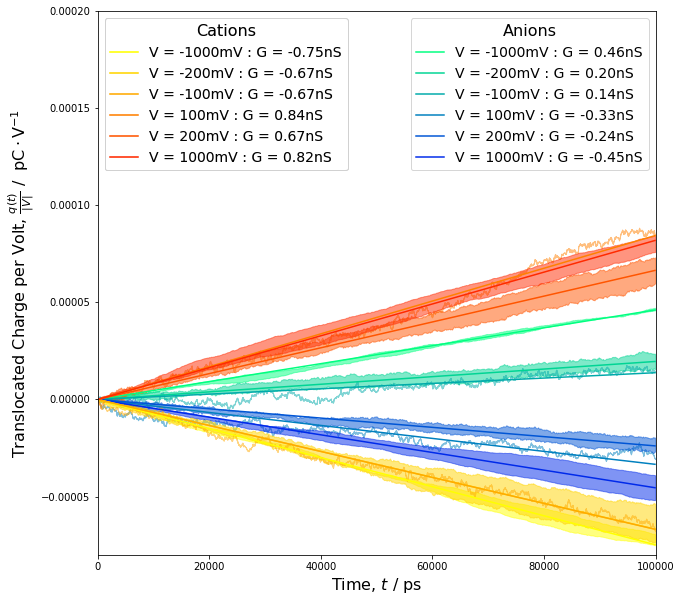
\includegraphics[scale=0.47]{conductance}
\caption{Conductance estimates $G$ from ensemble trajectories \\
for anions and cations across ompF under various applied voltages $V$ }
\label{fig:conductance}
\end{figure}

\subsection{Conductance estimates from molecular dynamics}
Classical force field molecular dynamics with an extental electric field was
used to estimate the conductance of ompF. The structure of ompF was embedded
in a lipid bilayer, surrounded by a water, Potassium $\mathrm{K^{+}}$ and
Chloride $\mathrm{Cl^{-}}$ ions. Simulations were run for up to 100ns with
external fields given by $V=\pm100\mathrm{mV},\pm200\mathrm{mV},\pm1\mathrm{V}$.
The translocated anionic and cationic charge $q(t)$ was recorded as a function of time.
Several trajectories for a given paramerer set where run to obtain a mean and
uncertainty. The cationic/anionic conductance $G_{\pm}$ was estimated via least squares according to
the formula
\begin{align}
	q(t)=G_{\pm}|V|t
\end{align}
Results summarised in Figure \ref{fig:conductance} show mean and standard
deviation for each trajectory ensemble. The claim of cationic selectivity
\cite{Benz1985} is supported as $|G_{+}|>|G_{-}|$ for all estimates and
applied voltages. Estimated conductances also share the same order of
magnitude as those reported in literature \cite{Benz1985}.

\bibliography{mendeley_v2}
\bibliographystyle{ieeetr}
\end{document}
